% igb-xdp-tx-stall-fix.tex — Technical book on the igb XDP/AF_XDP TX stall fix
% Author: Alex Dvoretsky
% License: CC BY 4.0
\documentclass[11pt,a4paper,openany]{book}

% ── Packages ──────────────────────────────────────────────────────────
\usepackage[T1]{fontenc}
\usepackage[utf8]{inputenc}
\usepackage{lmodern}
\usepackage[margin=1in,headheight=14pt]{geometry}
\usepackage{microtype}
\usepackage{graphicx}
\usepackage{xcolor}
\usepackage{listings}
\usepackage{tikz}
\usetikzlibrary{arrows.meta, positioning, calc, decorations.pathreplacing, fit}
\usepackage{hyperref}
\usepackage{bookmark}
\usepackage{fancyhdr}
\usepackage{titlesec}
\usepackage{enumitem}
\usepackage{booktabs}
\usepackage{longtable}
\usepackage{verbatim}
\usepackage{fancyvrb}
\usepackage{float}

% ── Hyperref setup ────────────────────────────────────────────────────
\hypersetup{
    colorlinks=true,
    linkcolor=blue!60!black,
    urlcolor=blue!70!black,
    citecolor=green!50!black,
    pdftitle={Fixing the igb XDP/AF\_XDP TX Queue Stall},
    pdfauthor={Alex Dvoretsky},
}

% ── Code listing style ───────────────────────────────────────────────
\definecolor{codebg}{RGB}{248,248,248}
\definecolor{codeframe}{RGB}{200,200,200}
\definecolor{codecomment}{RGB}{0,128,0}
\definecolor{codestring}{RGB}{163,21,21}
\definecolor{codekeyword}{RGB}{0,0,180}
\definecolor{diffadd}{RGB}{0,100,0}
\definecolor{diffrem}{RGB}{180,0,0}
\definecolor{diffhunk}{RGB}{0,0,160}

\lstdefinestyle{cstyle}{
    language=C,
    basicstyle=\ttfamily\small,
    keywordstyle=\color{codekeyword}\bfseries,
    commentstyle=\color{codecomment}\itshape,
    stringstyle=\color{codestring},
    backgroundcolor=\color{codebg},
    frame=single,
    rulecolor=\color{codeframe},
    numbers=left,
    numberstyle=\tiny\color{gray},
    numbersep=8pt,
    breaklines=true,
    breakatwhitespace=false,
    tabsize=8,
    showstringspaces=false,
    captionpos=b,
    xleftmargin=1.5em,
    framexleftmargin=1.5em,
    columns=flexible,
    morekeywords={u8,u16,u32,u64,s32,bool,__le32,__be16,dma_addr_t,
                  ktime_t,napi_struct,xsk_buff_pool,xdp_buff,
                  bpf_prog,igb_adapter,igb_ring,igb_q_vector,
                  igb_tx_buffer,net_device,netdev_queue,work_struct,
                  timer_list,netdev_bpf},
    literate={->}{{$\rightarrow$}}1,
}

\lstdefinestyle{diffstyle}{
    basicstyle=\ttfamily\small,
    backgroundcolor=\color{codebg},
    frame=single,
    rulecolor=\color{codeframe},
    breaklines=true,
    tabsize=8,
    showstringspaces=false,
    xleftmargin=0.5em,
    framexleftmargin=0.5em,
    columns=flexible,
    moredelim=[is][\color{diffadd}]{@@+}{+@@},
    moredelim=[is][\color{diffrem}]{@@-}{-@@},
    moredelim=[is][\color{diffhunk}\bfseries]{@@h}{h@@},
}

\lstdefinestyle{shellstyle}{
    basicstyle=\ttfamily\small,
    backgroundcolor=\color{codebg},
    frame=single,
    rulecolor=\color{codeframe},
    breaklines=true,
    showstringspaces=false,
    xleftmargin=0.5em,
    framexleftmargin=0.5em,
    columns=flexible,
}

\lstset{style=cstyle}

% ── Headers/footers ──────────────────────────────────────────────────
\pagestyle{fancy}
\fancyhf{}
\fancyhead[LE]{\leftmark}
\fancyhead[RO]{\rightmark}
\fancyfoot[C]{\thepage}
\renewcommand{\headrulewidth}{0.4pt}

% ── Chapter title format ─────────────────────────────────────────────
\titleformat{\chapter}[display]
    {\normalfont\huge\bfseries}
    {\chaptertitlename\ \thechapter}{20pt}{\Huge}

% ── Convenience macros ────────────────────────────────────────────────
\newcommand{\func}[1]{\texttt{#1()}}
\newcommand{\sym}[1]{\texttt{#1}}
\newcommand{\file}[1]{\texttt{#1}}
\newcommand{\flag}[1]{\texttt{#1}}
\newcommand{\state}[1]{\texttt{\_\_#1}}
\newcommand{\srcref}[2]{\texttt{#1:#2}}

% ══════════════════════════════════════════════════════════════════════
\begin{document}

% ── Title page ────────────────────────────────────────────────────────
\begin{titlepage}
\centering
\vspace*{2cm}
{\Huge\bfseries Fixing the igb Driver\\[0.3em]
XDP/AF\_XDP TX Queue Stall\par}
\vspace{1.5cm}
{\Large\itshape A Deep Dive into NAPI Polling, \texttt{napi\_disable()},\\
and the Redundant \texttt{napi\_synchronize()} in the Linux Kernel\par}
\vspace{2cm}
{\Large Alex Dvoretsky\par}
\vspace{1cm}
{\large March 2026\par}
\vfill
{\normalsize
Based on a single-line patch for the Linux kernel \texttt{igb} driver\\
targeting the Intel I210/I211 Gigabit Ethernet controllers.\\[1em]
Kernel version: 6.17 \quad|\quad Patch version: v2}
\end{titlepage}

% ── Front matter ──────────────────────────────────────────────────────
\frontmatter
\tableofcontents

% ══════════════════════════════════════════════════════════════════════
%  MAIN MATTER
% ══════════════════════════════════════════════════════════════════════
\mainmatter

% ======================================================================
\chapter{Introduction}
\label{ch:intro}
% ======================================================================

\section{The Problem}

Consider a typical deployment scenario: an Intel I210 Gigabit Ethernet
controller driven by the \texttt{igb} kernel module, with an XDP program
attached and an AF\_XDP zero-copy application processing packets at high
speed.  Everything works perfectly---until the AF\_XDP application is
killed.

\begin{lstlisting}[style=shellstyle]
$ kill -9 $AF_XDP_PID
\end{lstlisting}

Within five seconds, the kernel logs an ominous message:

\begin{lstlisting}[style=shellstyle]
NETDEV WATCHDOG: CPU: 3: enp8s0 (igb): transmit queue 0 timed out 5008 ms
\end{lstlisting}

The interface becomes completely unresponsive.  No packets are
transmitted or received.  Pings fail, SSH sessions hang, and the only
recovery is to reload the \texttt{igb} module or reboot the machine.

The root cause is a redundant \func{napi\_synchronize} call in
\func{igb\_down}.  When the AF\_XDP buffer pool is destroyed, the
zero-copy RX poll function enters an infinite loop, returning full
budget on every cycle.  \func{napi\_synchronize} spins waiting for
this poll to finish---but it never will.  The subsequent
\func{napi\_disable}, which \emph{can} break the loop via the
\flag{NAPI\_STATE\_DISABLE} mechanism, never gets a chance to run.

The fix is a single line: remove the \func{napi\_synchronize} call.

\section{Scope of This Book}

This book explains the Linux kernel subsystems that interact to produce
this bug, then walks through the fix and why it is correct.  Each
chapter builds the prerequisite knowledge:

\begin{description}[style=nextline]
\item[Chapter~\ref{ch:napi}] explains the NAPI polling architecture---how
    interrupts are coalesced into poll cycles, how poll completion works,
    and the critical difference between \func{napi\_synchronize} and
    \func{napi\_disable}.
\item[Chapter~\ref{ch:afxdp}] covers AF\_XDP zero-copy in the \texttt{igb}
    driver: the buffer pool, the ZC receive path, and what happens when
    the pool is destroyed.
\item[Chapter~\ref{ch:xdp-lifecycle}] traces the lifecycle of an XDP
    program: how \func{igb\_xdp\_setup} installs and removes programs, and
    how \func{igb\_close}/\func{igb\_open} perform the device reset.
\item[Chapter~\ref{ch:watchdog}] describes the TX watchdog timer---the
    visible symptom of the bug, though not its root cause.
\item[Chapter~\ref{ch:fix}] analyzes the v2 fix: why removing
    \func{napi\_synchronize} is correct and sufficient.
\item[Chapter~\ref{ch:evolution}] traces the evolution from an initial
    3-patch v1 series to the minimal v2 fix, following reviewer feedback
    from Intel's Maciej Fijalkowski.
\end{description}

\section{Affected Hardware}

The bug affects all hardware supported by the \texttt{igb} driver that has
AF\_XDP zero-copy support.  In practice, this means the Intel I210 and
I211 controllers (PCI device IDs \texttt{0x1533} and \texttt{0x1539}),
which are common on embedded and server platforms.

The testing for this patch was performed on an Intel I210 (PCI
address \texttt{0000:08:00.0}) using the \texttt{igb} driver version
shipped with Linux 6.17.

% ======================================================================
\chapter{NAPI Polling Architecture}
\label{ch:napi}
% ======================================================================

NAPI (New API) is the Linux kernel's mechanism for efficient network
packet processing.  Rather than handling every incoming packet via a
hardware interrupt, NAPI coalesces interrupts into \emph{poll cycles}
where the driver processes packets in batches.

Understanding NAPI is essential for this book because the TX stall bug
is, at its core, a NAPI poll loop that never terminates---and the fix
relies on understanding how \func{napi\_disable} breaks such loops from
the inside.

\section{The Interrupt-to-Poll Transition}

The lifecycle of a NAPI poll cycle has four phases:

\begin{enumerate}
\item \textbf{Hardware interrupt fires.}  The NIC signals that packets
    are available (or TX descriptors have been completed).
\item \textbf{Driver schedules NAPI.}  The interrupt handler calls
    \func{napi\_schedule}, which sets the \flag{NAPI\_STATE\_SCHED} bit
    and adds the NAPI instance to the per-CPU poll list.
\item \textbf{Softirq runs the poll function.}  The \texttt{NET\_RX\_SOFTIRQ}
    handler calls the driver's \sym{poll} callback with a
    \texttt{budget} (typically 64 packets).
\item \textbf{Poll completes or re-arms.}  If the driver processed fewer
    packets than the budget (\texttt{work\_done < budget}), it calls
    \func{napi\_complete\_done} to signal completion and re-enable
    interrupts.  If it consumed the full budget, it returns
    \texttt{budget} and NAPI will call it again.
\end{enumerate}

\begin{figure}[H]
\centering
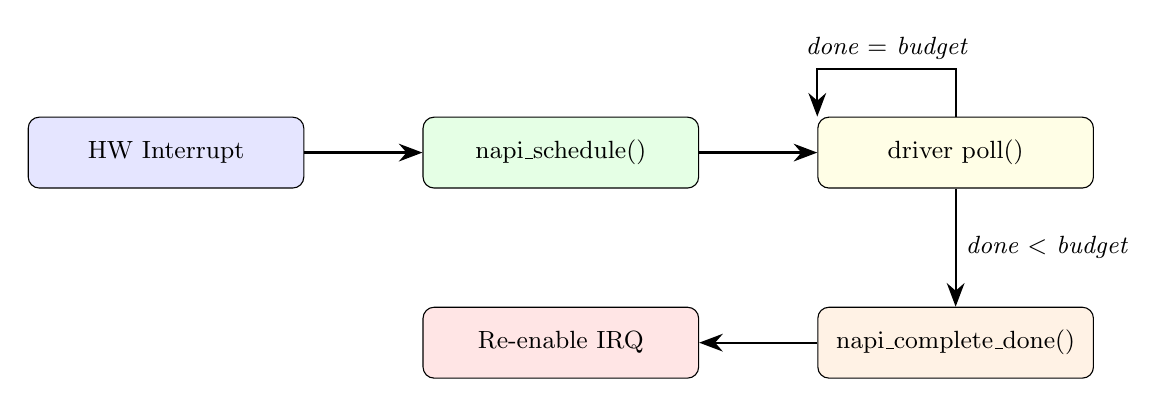
\begin{tikzpicture}[
    box/.style={draw, rounded corners, minimum width=3.5cm, minimum height=0.9cm,
                text centered, font=\small},
    arr/.style={-{Stealth[length=3mm]}, thick},
    node distance=1.5cm
]
\node[box, fill=blue!10] (irq) {HW Interrupt};
\node[box, fill=green!10, right=of irq] (sched) {napi\_schedule()};
\node[box, fill=yellow!10, right=of sched] (poll) {driver poll()};
\node[box, fill=orange!10, below=of poll] (complete) {napi\_complete\_done()};
\node[box, fill=red!10, below=of sched] (rearm) {Re-enable IRQ};

\draw[arr] (irq) -- (sched);
\draw[arr] (sched) -- (poll);
\draw[arr] (poll) -- node[right, font=\small\itshape] {done $<$ budget} (complete);
\draw[arr] (complete) -- (rearm);
\draw[arr] (poll.north) -- ++(0,0.6) -| node[above, pos=0.25, font=\small\itshape]
    {done $=$ budget} (poll.north west);
\end{tikzpicture}
\caption{NAPI poll lifecycle.  The poll function is called repeatedly
  as long as it returns \texttt{budget}; it exits the cycle by returning
  less than \texttt{budget}.}
\label{fig:napi-lifecycle}
\end{figure}

\section{The \texttt{napi\_struct}}

Each NAPI instance is represented by a \sym{napi\_struct}:

\begin{lstlisting}[caption={Simplified \texttt{napi\_struct} (include/linux/netdevice.h)}]
struct napi_struct {
    unsigned long       state;
    struct list_head    poll_list;
    int                 weight;
    int                 (*poll)(struct napi_struct *, int);
    struct net_device   *dev;
    struct hrtimer      timer;
    /* ... */
};
\end{lstlisting}

The \sym{state} field is a bitmask of flags.  The ones relevant to
this book are:

\begin{table}[H]
\centering
\begin{tabular}{lp{10cm}}
\toprule
\textbf{Flag} & \textbf{Meaning} \\
\midrule
\flag{NAPI\_STATE\_SCHED} &
    NAPI is scheduled for polling.  Set by \func{napi\_schedule\_prep},
    cleared by \func{napi\_complete\_done}.  \\
\flag{NAPI\_STATE\_MISSED} &
    New work arrived while NAPI was completing.  If
    \func{napi\_complete\_done} sees this flag, it re-schedules the
    poll instead of completing.  \\
\flag{NAPI\_STATE\_DISABLE} &
    NAPI is being disabled.  Set by \func{napi\_disable}.
    \func{napi\_schedule\_prep} will refuse to schedule when this is set.
    Crucially, \func{\_\_napi\_poll} checks this flag after every
    full-budget poll return and forces completion if set.  \\
\bottomrule
\end{tabular}
\caption{Key NAPI state flags.}
\label{tab:napi-flags}
\end{table}

\section{The Budget Contract}
\label{sec:budget-contract}

The NAPI budget contract is the fundamental agreement between the kernel
and the driver's poll function:

\begin{itemize}
\item The kernel calls \texttt{poll(napi, budget)} with a positive
    budget (default weight is 64).
\item If the driver returns a value \textbf{equal to} \texttt{budget},
    the kernel assumes there is more work and will call \texttt{poll}
    again.
\item If the driver returns a value \textbf{less than} \texttt{budget},
    the driver must have called \func{napi\_complete\_done} to signal
    that the poll cycle is finished.
\end{itemize}

This contract is critical: if a poll function \emph{always} returns
\texttt{budget} without ever returning a smaller value, NAPI will keep
polling forever.  This is exactly what happens in the bug we are fixing.

\section{\texttt{napi\_complete\_done()}: The Completion CAS Loop}
\label{sec:napi-complete-done}

\func{napi\_complete\_done} is the function that transitions a NAPI
instance from the ``polling'' state back to the ``idle'' state.  Its
implementation contains an atomic compare-and-swap (CAS) loop that
handles the \flag{MISSED} flag:

\begin{lstlisting}[caption={\texttt{napi\_complete\_done()} core logic (net/core/dev.c)},
    label=lst:napi-complete-done]
bool napi_complete_done(struct napi_struct *n, int work_done)
{
    unsigned long flags, val, new, timeout = 0;
    bool ret = true;

    if (unlikely(n->state & (NAPIF_STATE_NPSVC |
                             NAPIF_STATE_IN_BUSY_POLL)))
        return false;

    /* ... GRO flush, poll_list removal ... */

    val = READ_ONCE(n->state);
    do {
        WARN_ON_ONCE(!(val & NAPIF_STATE_SCHED));

        new = val & ~(NAPIF_STATE_MISSED | NAPIF_STATE_SCHED |
                      NAPIF_STATE_SCHED_THREADED |
                      NAPIF_STATE_PREFER_BUSY_POLL);

        /* If MISSED was set, keep SCHED set for one more poll */
        new |= (val & NAPIF_STATE_MISSED) /
               NAPIF_STATE_MISSED * NAPIF_STATE_SCHED;
    } while (!try_cmpxchg(&n->state, &val, new));

    if (unlikely(val & NAPIF_STATE_MISSED)) {
        __napi_schedule(n);
        return false;
    }

    /* ... hrtimer for GRO ... */
    return ret;
}
\end{lstlisting}

The key insight is the \flag{MISSED} flag re-scheduling logic.  When
another CPU (or the driver itself) sets \flag{MISSED} during the CAS
window, \func{napi\_complete\_done} sees it and re-schedules NAPI
instead of completing.

\section{\texttt{napi\_synchronize()}: The Passive Wait}
\label{sec:napi-synchronize}

\func{napi\_synchronize} is a simple busy-wait that spins until the
\flag{NAPI\_STATE\_SCHED} bit is clear:

\begin{lstlisting}[caption={\texttt{napi\_synchronize()} (include/linux/netdevice.h)}]
static inline void napi_synchronize(const struct napi_struct *n)
{
    if (IS_ENABLED(CONFIG_SMP))
        while (test_bit(NAPI_STATE_SCHED, &n->state))
            msleep(1);
    else
        barrier();
}
\end{lstlisting}

This function is purely passive: it waits for the poll function to
finish on its own.  It does \emph{not} set any flags, does not signal
the poll function, and does not prevent future scheduling.  It simply
polls the \flag{NAPI\_STATE\_SCHED} bit with a 1\,ms sleep between
iterations.

\textbf{Critical property:} if the poll function never returns
\texttt{done < budget}, then \func{napi\_complete\_done} is never called,
\flag{NAPI\_STATE\_SCHED} is never cleared, and
\func{napi\_synchronize} \textbf{spins forever}.  This is not a
deadlock---it is a livelock: both the poll function and the synchronize
caller are making progress (burning CPU), but neither can terminate.

\subsection{Historical Context}

The \func{napi\_synchronize} call in \func{igb\_down} was introduced in
commit \texttt{41f149a285da} (``igb: Fix possible panic caused by Rx
traffic arrival while interface is down'').  The intent was to ensure
that no NAPI poll callback was actively running before disabling NAPI,
so that the poll function would not access freed resources.

At the time this commit was written (2009), the NAPI subsystem's
\func{napi\_disable} was less sophisticated.  The
\flag{NAPI\_STATE\_DISABLE} mechanism and the
\func{napi\_disable\_pending} check in \func{\_\_napi\_poll} were
later refinements that made the explicit synchronize unnecessary.

\section{\texttt{napi\_disable()}: The Active Shutdown}
\label{sec:napi-disable}

\func{napi\_disable} is the intended way to shut down a NAPI instance
during device teardown.  Unlike \func{napi\_synchronize}, it actively
\emph{signals} the poll function to stop:

\begin{lstlisting}[caption={\texttt{napi\_disable()} (net/core/dev.c)},
    label=lst:napi-disable]
void napi_disable(struct napi_struct *n)
{
    unsigned long val, new;

    might_sleep();
    set_bit(NAPI_STATE_DISABLE, &n->state);

    val = READ_ONCE(n->state);
    do {
        while (val & NAPIF_STATE_SCHED) {
            usleep_range(20, 200);
            val = READ_ONCE(n->state);
        }

        new = val | NAPIF_STATE_SCHED |
                    NAPIF_STATE_NPSVC;
        new &= ~(NAPIF_STATE_DISABLE |
                  NAPIF_STATE_PREFER_BUSY_POLL);
    } while (!try_cmpxchg(&n->state, &val, new));
}
\end{lstlisting}

The key steps are:

\begin{enumerate}
\item \textbf{Set \flag{NAPI\_STATE\_DISABLE}.}  This is the signal.
    Once set, the NAPI core will intervene to break any stuck poll loop
    (see Section~\ref{sec:napi-poll-check}).
\item \textbf{Wait for \flag{NAPI\_STATE\_SCHED} to clear.}  Like
    \func{napi\_synchronize}, this waits for the current poll to finish.
    But because \flag{NAPI\_STATE\_DISABLE} is now set, the NAPI core
    will \emph{force} the poll to finish (see below).
\item \textbf{Atomically set \flag{SCHED} and \flag{NPSVC}.}  This
    prevents any future scheduling---the NAPI instance is now
    permanently disabled until \func{napi\_enable} is called.
\end{enumerate}

\textbf{The crucial difference:} \func{napi\_synchronize} waits
passively for \flag{SCHED} to clear.  \func{napi\_disable} \emph{also}
waits---but it first sets \flag{DISABLE}, which triggers the forced
completion mechanism in \func{\_\_napi\_poll}.  This is why
\func{napi\_disable} can handle a stuck poll loop and
\func{napi\_synchronize} cannot.

\section{\texttt{\_\_napi\_poll()}: The Forced Completion Mechanism}
\label{sec:napi-poll-check}

The NAPI core function \func{\_\_napi\_poll} is where the magic happens.
After calling the driver's poll function, it checks whether a disable
is pending:

\begin{lstlisting}[caption={\texttt{\_\_napi\_poll()} forced completion (net/core/dev.c)},
    label=lst:napi-poll-check]
static int __napi_poll(struct napi_struct *n, bool *repoll)
{
    int work, weight;

    weight = n->weight;
    work = n->poll(n, weight);

    if (likely(work < weight))
        return work;

    /* Driver returned full budget.
     * Normally we would repoll, but check for disable first. */
    if (unlikely(napi_disable_pending(n))) {
        napi_complete(n);  /* forces SCHED clear */
        return work;
    }

    /* ... busy poll, time limit checks ... */

    *repoll = true;
    return work;
}
\end{lstlisting}

\func{napi\_disable\_pending} simply checks the \flag{NAPI\_STATE\_DISABLE}
bit:

\begin{lstlisting}[caption={\texttt{napi\_disable\_pending()} (include/linux/netdevice.h)}]
static inline bool napi_disable_pending(struct napi_struct *n)
{
    return test_bit(NAPI_STATE_DISABLE, &n->state);
}
\end{lstlisting}

When the poll function returns full budget \emph{and}
\flag{NAPI\_STATE\_DISABLE} is set, \func{\_\_napi\_poll} calls
\func{napi\_complete} to force-clear \flag{NAPI\_STATE\_SCHED}.  This
breaks the infinite loop:

\begin{enumerate}
\item \func{napi\_disable} sets \flag{NAPI\_STATE\_DISABLE}.
\item The poll function runs and returns full budget (the stuck loop).
\item \func{\_\_napi\_poll} sees \func{napi\_disable\_pending} is true.
\item \func{napi\_complete} clears \flag{NAPI\_STATE\_SCHED}.
\item \func{napi\_disable} sees \flag{SCHED} clear and proceeds to
    finalize the shutdown.
\end{enumerate}

This mechanism was designed precisely for situations where a poll
function is stuck returning full budget.  It allows \func{napi\_disable}
to reliably shut down any NAPI instance, regardless of what the poll
function is doing.

\begin{figure}[H]
\centering
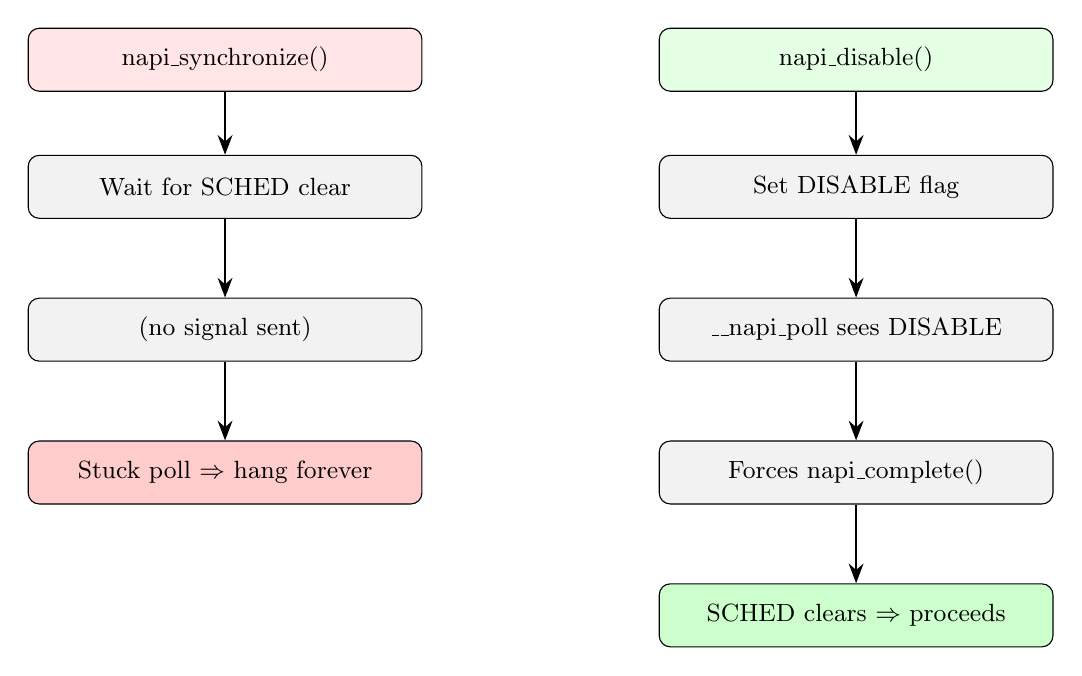
\begin{tikzpicture}[
    box/.style={draw, rounded corners, minimum width=5cm, minimum height=0.8cm,
                text centered, font=\small},
    arr/.style={-{Stealth[length=2.5mm]}, thick},
    node distance=1cm
]
\node[box, fill=red!10] (sync) {napi\_synchronize()};
\node[box, fill=green!10, right=3cm of sync] (disable) {napi\_disable()};

\node[box, fill=gray!10, below=0.8cm of sync] (sync1) {Wait for SCHED clear};
\node[box, fill=gray!10, below=of sync1] (sync2) {(no signal sent)};
\node[box, fill=red!20, below=of sync2] (sync3) {Stuck poll $\Rightarrow$ hang forever};

\node[box, fill=gray!10, below=0.8cm of disable] (dis1) {Set DISABLE flag};
\node[box, fill=gray!10, below=of dis1] (dis2) {\_\_napi\_poll sees DISABLE};
\node[box, fill=gray!10, below=of dis2] (dis3) {Forces napi\_complete()};
\node[box, fill=green!20, below=of dis3] (dis4) {SCHED clears $\Rightarrow$ proceeds};

\draw[arr] (sync) -- (sync1);
\draw[arr] (sync1) -- (sync2);
\draw[arr] (sync2) -- (sync3);

\draw[arr] (disable) -- (dis1);
\draw[arr] (dis1) -- (dis2);
\draw[arr] (dis2) -- (dis3);
\draw[arr] (dis3) -- (dis4);
\end{tikzpicture}
\caption{Comparison of \texttt{napi\_synchronize()} vs
  \texttt{napi\_disable()} when a poll function is stuck returning full
  budget.  Only \texttt{napi\_disable()} can break the loop.}
\label{fig:sync-vs-disable}
\end{figure}

\section{\texttt{igb\_poll()}: The igb Driver's NAPI Callback}
\label{sec:igb-poll}

The \texttt{igb} driver registers \func{igb\_poll} as the NAPI poll
callback.  It processes TX completions first, then RX packets:

\begin{lstlisting}[caption={\texttt{igb\_poll()} (igb\_main.c:8280)},
    label=lst:igb-poll]
static int igb_poll(struct napi_struct *napi, int budget)
{
    struct igb_q_vector *q_vector = container_of(napi,
                         struct igb_q_vector, napi);
    struct xsk_buff_pool *xsk_pool;
    bool clean_complete = true;
    int work_done = 0;

    if (q_vector->tx.ring)
        clean_complete = igb_clean_tx_irq(q_vector, budget);

    if (q_vector->rx.ring) {
        int cleaned;

        xsk_pool = READ_ONCE(q_vector->rx.ring->xsk_pool);
        cleaned = xsk_pool ?
            igb_clean_rx_irq_zc(q_vector, xsk_pool, budget) :
            igb_clean_rx_irq(q_vector, budget);

        work_done += cleaned;
        if (cleaned >= budget)
            clean_complete = false;
    }

    if (!clean_complete)
        return budget;

    if (likely(napi_complete_done(napi, work_done)))
        igb_ring_irq_enable(q_vector);

    return work_done;
}
\end{lstlisting}

The decision tree is:

\begin{enumerate}
\item If \func{igb\_clean\_tx\_irq} returns \texttt{false} (more TX work),
    \texttt{clean\_complete} is set to \texttt{false}.
\item If the RX cleaner returns \texttt{budget} or more,
    \texttt{clean\_complete} is set to \texttt{false}.
\item If \texttt{clean\_complete} is \texttt{false}, return
    \texttt{budget} without calling \func{napi\_complete\_done}---NAPI
    will call us again.
\item Otherwise, call \func{napi\_complete\_done} and re-enable
    interrupts.
\end{enumerate}

\section{The \texttt{\_\_IGB\_DOWN} Early-Exit Pattern}
\label{sec:igb-down-pattern}

\func{igb\_clean\_tx\_irq} begins with an early-exit check:

\begin{lstlisting}[caption={\texttt{\_\_IGB\_DOWN} check in \texttt{igb\_clean\_tx\_irq()} (igb\_main.c:8344)},
    label=lst:tx-irq-down-check]
static bool igb_clean_tx_irq(struct igb_q_vector *q_vector,
                             int napi_budget)
{
    struct igb_adapter *adapter = q_vector->adapter;
    /* ... */

    if (test_bit(__IGB_DOWN, &adapter->state))
        return true;

    /* ... process TX completions ... */
}
\end{lstlisting}

When the adapter is going down (\flag{\_\_IGB\_DOWN} is set by
\func{igb\_down}), \func{igb\_clean\_tx\_irq} returns \texttt{true}
immediately.  In the context of \func{igb\_poll}, \texttt{true} means
``TX work is complete'' (sets \texttt{clean\_complete = true}).

This pattern is relevant because \func{igb\_clean\_rx\_irq\_zc}
\emph{lacks} the same check---but as we will see in
Chapter~\ref{ch:fix}, the v2 fix makes such a check unnecessary by
removing the \func{napi\_synchronize} that would hang.


% ======================================================================
\chapter{AF\_XDP Zero-Copy in igb}
\label{ch:afxdp}
% ======================================================================

AF\_XDP is a high-performance packet I/O mechanism that allows
user-space applications to send and receive network packets with minimal
kernel overhead.  When used in \emph{zero-copy mode}, the NIC's DMA
engine reads and writes directly to user-space memory, bypassing the
kernel's \texttt{sk\_buff} allocation entirely.

\section{AF\_XDP Architecture}

An AF\_XDP socket operates on a shared memory region called a UMEM
(User Memory for Efficient Mapping).  The UMEM is divided into
fixed-size frames, and four ring buffers coordinate frame ownership
between the kernel and user-space:

\begin{table}[H]
\centering
\begin{tabular}{lll}
\toprule
\textbf{Ring} & \textbf{Direction} & \textbf{Purpose} \\
\midrule
Fill Queue (FQ)      & User $\to$ Kernel & User provides empty frames for RX \\
Completion Queue (CQ)& Kernel $\to$ User & Kernel returns frames after TX \\
RX Ring              & Kernel $\to$ User & Kernel delivers received packets \\
TX Ring              & User $\to$ Kernel & User submits packets for TX \\
\bottomrule
\end{tabular}
\caption{AF\_XDP ring buffers.}
\end{table}

In zero-copy mode, the kernel maps the UMEM directly into the NIC's DMA
address space.  The driver programs the NIC's RX descriptor ring with
DMA addresses pointing into the UMEM, so received packets land directly
in user-space memory.

\section{Zero-Copy vs.\ Copy Mode}

\begin{description}
\item[Copy mode] The kernel receives packets into its own buffers via
    the normal RX path, then copies the packet data into the AF\_XDP
    socket's UMEM.  This adds a \texttt{memcpy} per packet but works
    with any driver.
\item[Zero-copy mode] The driver is aware of AF\_XDP and programs the
    NIC to DMA directly into the UMEM.  This eliminates the copy but
    requires explicit driver support.  The \texttt{igb} driver gained
    zero-copy support in commit \texttt{2c6196013f84} (``igb: Add AF\_XDP
    zero-copy Rx support'').
\end{description}

\section{The XSK Buffer Pool}

The kernel-side representation of the UMEM for a particular queue is
the \sym{xsk\_buff\_pool}.  It is created when a user-space application
binds an AF\_XDP socket to a specific queue:

\begin{lstlisting}[caption={XSK pool reference in \texttt{igb\_ring} (igb.h)}]
struct igb_ring {
    /* ... */
    struct xsk_buff_pool *xsk_pool;
    /* ... */
    union {
        struct igb_rx_buffer *rx_buffer_info;
        struct xdp_buff **rx_buffer_info_zc;
    };
    /* ... */
};
\end{lstlisting}

When the pool is present, the ring uses \sym{rx\_buffer\_info\_zc} (an
array of \sym{xdp\_buff} pointers) instead of the normal
\sym{rx\_buffer\_info}.  Buffer allocation uses \func{xsk\_buff\_alloc}
or \func{xsk\_buff\_alloc\_batch} to obtain frames from the Fill Queue.

\textbf{Key observation:} when the AF\_XDP application dies, the pool
is destroyed.  After that point, \func{xsk\_buff\_alloc} returns
\texttt{NULL}---there are no more frames to allocate.

\section{\texttt{igb\_clean\_rx\_irq\_zc()}: The Zero-Copy RX Path}
\label{sec:clean-rx-zc}

\func{igb\_clean\_rx\_irq\_zc} is the RX poll function used when a ZC
pool is active on a ring.  It is selected by \func{igb\_poll} based on
the presence of \sym{xsk\_pool}:

\begin{lstlisting}[caption={ZC RX path selection in \texttt{igb\_poll()} (igb\_main.c:8300)}]
xsk_pool = READ_ONCE(q_vector->rx.ring->xsk_pool);
cleaned = xsk_pool ?
    igb_clean_rx_irq_zc(q_vector, xsk_pool, budget) :
    igb_clean_rx_irq(q_vector, budget);
\end{lstlisting}

The function processes received packets from the descriptor ring,
runs them through the XDP program, and allocates replacement buffers
from the pool:

\begin{lstlisting}[caption={\texttt{igb\_clean\_rx\_irq\_zc()} (igb\_xsk.c:341), simplified},
    label=lst:clean-rx-zc]
int igb_clean_rx_irq_zc(struct igb_q_vector *q_vector,
                        struct xsk_buff_pool *xsk_pool,
                        const int budget)
{
    struct igb_adapter *adapter = q_vector->adapter;
    struct igb_ring *rx_ring = q_vector->rx.ring;
    unsigned int total_packets = 0;
    /* ... */

    xdp_prog = READ_ONCE(rx_ring->xdp_prog);

    while (likely(total_packets < budget)) {
        /* Try to read a completed RX descriptor */
        rx_desc = IGB_RX_DESC(rx_ring, ntc);
        size = le16_to_cpu(rx_desc->wb.upper.length);
        if (!size)
            break;     /* no more completed descriptors */

        /* ... process the packet via XDP ... */
        total_packets++;
    }

    /* ... update ring pointers ... */

    /* Try to refill the ring with new buffers */
    entries_to_alloc = igb_desc_unused(rx_ring);
    if (entries_to_alloc >= IGB_RX_BUFFER_WRITE)
        failure |= !igb_alloc_rx_buffers_zc(rx_ring, xsk_pool,
                                            entries_to_alloc);

    if (xsk_uses_need_wakeup(xsk_pool)) {
        /* ... wakeup handling ... */
        return (int)total_packets;
    }
    return failure ? budget : (int)total_packets;
}
\end{lstlisting}

\subsection{The Return Value Semantics}

The return value of \func{igb\_clean\_rx\_irq\_zc} determines
whether NAPI considers the poll complete:

\begin{itemize}
\item If \texttt{total\_packets < budget}, NAPI calls
    \func{napi\_complete\_done} and the poll cycle ends.
\item If \texttt{total\_packets >= budget} (or \texttt{failure}
    returns \texttt{budget}), NAPI continues polling.
\end{itemize}

The \texttt{failure} flag is set when buffer allocation fails---meaning
the Fill Queue is empty.  In that case, the function returns
\texttt{budget} to request another poll cycle, hoping that the user-space
application will refill the Fill Queue.

\subsection{What Happens When the Pool Is Destroyed}

When the AF\_XDP application dies:
\begin{enumerate}
\item The XSK buffer pool is destroyed.
\item \func{xsk\_buff\_alloc\_batch} returns 0 buffers---the Fill Queue
    is gone.
\item \func{igb\_alloc\_rx\_buffers\_zc} returns \texttt{false}
    (failure), so \texttt{failure = true}.
\item There are no completed RX descriptors (the NIC has no buffers
    to write to), so the \texttt{while} loop processes 0 packets.
\item \texttt{total\_packets = 0}, but \texttt{failure = true}, so the
    function returns \texttt{budget}.
\item Back in \func{igb\_poll}: \texttt{cleaned >= budget} $\Rightarrow$
    \texttt{clean\_complete = false} $\Rightarrow$ return \texttt{budget}
    without calling \func{napi\_complete\_done}.
\item NAPI re-schedules the poll.  Go to step 2.
\end{enumerate}

This creates an \textbf{infinite NAPI poll loop}: the function keeps
returning \texttt{budget} because it cannot allocate buffers, and NAPI
keeps calling it because it thinks there is more work to do.

This infinite loop is the trigger condition for the bug.  However, as we
will see, the infinite loop \emph{alone} does not cause the TX stall.
The problem is that \func{igb\_down} calls \func{napi\_synchronize}
\emph{before} \func{napi\_disable}.  \func{napi\_synchronize} cannot
break the loop; \func{napi\_disable} can.  By the time
\func{napi\_disable} would run, \func{igb\_down} is already stuck.

\section{Buffer Pool Lifecycle}

The full lifecycle of a zero-copy buffer pool:

\begin{enumerate}
\item \textbf{Creation.}  User-space creates an AF\_XDP socket and binds
    it to queue $N$.  The kernel creates an \sym{xsk\_buff\_pool} and
    stores it in \texttt{adapter->rx\_ring[N]->xsk\_pool}.
\item \textbf{Active use.}  The driver's ZC RX/TX paths use the pool to
    allocate and complete buffers.
\item \textbf{Destruction.}  The AF\_XDP socket is closed (either
    normally or because the process dies).  The pool is destroyed, and
    \texttt{xsk\_pool} is set to \texttt{NULL}---but not necessarily
    before the NAPI poll function has already read the old pointer.
\end{enumerate}

The race between pool destruction and NAPI polling is what triggers
the infinite loop: \func{igb\_poll} reads a non-NULL \sym{xsk\_pool}
pointer and calls \func{igb\_clean\_rx\_irq\_zc}, but by the time the
function tries to allocate buffers, the pool is already gone.


% ======================================================================
\chapter{XDP Program Lifecycle and Device Reset}
\label{ch:xdp-lifecycle}
% ======================================================================

\section{\texttt{igb\_xdp\_setup()}: Installing and Removing XDP Programs}
\label{sec:xdp-setup}

The netdev core calls \func{igb\_xdp\_setup} when an XDP program is
attached to or detached from the interface.  The function handles two
cases:

\begin{description}
\item[Program replacement] (e.g., updating the XDP program without
    changing modes): the new program is atomically swapped in without
    a reset.
\item[Mode transition] (XDP $\to$ non-XDP or non-XDP $\to$ XDP): the
    device must be reset because the ring layout changes.
\end{description}

\begin{lstlisting}[caption={\texttt{igb\_xdp\_setup()} (igb\_main.c:2890)},
    label=lst:xdp-setup]
static int igb_xdp_setup(struct net_device *dev,
                         struct netdev_bpf *bpf)
{
    struct igb_adapter *adapter = netdev_priv(dev);
    struct bpf_prog *prog = bpf->prog, *old_prog;
    bool running = netif_running(dev);
    bool need_reset;

    /* ... frame size validation ... */

    old_prog = xchg(&adapter->xdp_prog, prog);
    need_reset = (!!prog != !!old_prog);

    if (need_reset && running) {
        igb_close(dev);
    } else {
        for (i = 0; i < adapter->num_rx_queues; i++)
            (void)xchg(&adapter->rx_ring[i]->xdp_prog,
                adapter->xdp_prog);
    }

    if (old_prog)
        bpf_prog_put(old_prog);

    if (!need_reset)
        return 0;

    /* ... xdp_features update ... */

    if (running)
        igb_open(dev);

    return 0;
}
\end{lstlisting}

When a mode transition occurs on a running device, the function calls
\func{igb\_close} followed by \func{igb\_open}.  This is a complete
device teardown and reinitialization---the most disruptive operation
the driver performs.

\section{\texttt{igb\_close()}: Tearing Down the Device}

\func{igb\_close} is the network device's close callback
(\texttt{ndo\_stop}).  It delegates to \func{\_\_igb\_close}:

\begin{lstlisting}[caption={\texttt{igb\_close()} and \texttt{\_\_igb\_close()} (igb\_main.c:4259)}]
static int __igb_close(struct net_device *netdev,
                       bool suspending)
{
    struct igb_adapter *adapter = netdev_priv(netdev);

    igb_down(adapter);
    igb_free_irq(adapter);
    igb_free_all_tx_resources(adapter);
    igb_free_all_rx_resources(adapter);
    /* ... */
    return 0;
}
\end{lstlisting}

The real work happens in \func{igb\_down}.

\section{\texttt{igb\_down()}: The Shutdown Sequence}
\label{sec:igb-down}

\func{igb\_down} is the core shutdown function.  Understanding its
sequence is essential for understanding the bug:

\begin{lstlisting}[caption={\texttt{igb\_down()} (igb\_main.c:2170), before the fix},
    label=lst:igb-down]
void igb_down(struct igb_adapter *adapter)
{
    struct net_device *netdev = adapter->netdev;
    struct e1000_hw *hw = &adapter->hw;

    /* (1) Signal shutdown */
    set_bit(__IGB_DOWN, &adapter->state);

    /* (2) Disable HW RX */
    rctl = rd32(E1000_RCTL);
    wr32(E1000_RCTL, rctl & ~E1000_RCTL_EN);

    /* (3) Stop TX queues, disable HW TX */
    netif_carrier_off(netdev);
    netif_tx_stop_all_queues(netdev);
    tctl = rd32(E1000_TCTL);
    tctl &= ~E1000_TCTL_EN;
    wr32(E1000_TCTL, tctl);
    wrfl();
    usleep_range(10000, 11000);

    /* (4) Disable interrupts */
    igb_irq_disable(adapter);

    /* (5) Wait for NAPI, then disable it */
    for (i = 0; i < adapter->num_q_vectors; i++) {
        if (adapter->q_vector[i]) {
            napi_synchronize(           /* <-- THE BUG */
                &adapter->q_vector[i]->napi);
            igb_set_queue_napi(adapter, i, NULL);
            napi_disable(
                &adapter->q_vector[i]->napi);
        }
    }

    /* (6) Cancel timers, update stats, reset HW */
    timer_delete_sync(&adapter->watchdog_timer);
    /* ... */
    igb_reset(adapter);

    /* (7) Clean all rings */
    igb_clean_all_tx_rings(adapter);
    igb_clean_all_rx_rings(adapter);
}
\end{lstlisting}

The sequence has a clear dependency chain:

\begin{enumerate}
\item \textbf{Set \flag{\_\_IGB\_DOWN}} (step 1) to signal all paths that
    the adapter is going down.
\item \textbf{Disable hardware} (steps 2--4) to stop new packets and
    interrupts.
\item \textbf{Wait for NAPI} (step 5): \func{napi\_synchronize} blocks
    until the current poll cycle completes, then \func{napi\_disable}
    prevents future scheduling.
\item \textbf{Clean up} (steps 6--7) now that no concurrent access is
    possible.
\end{enumerate}

\textbf{The bug is in step 5.}  \func{napi\_synchronize} is called
\emph{before} \func{napi\_disable}.  If the poll function is stuck in an
infinite loop (as with the ZC bug described in
Section~\ref{sec:clean-rx-zc}), \func{napi\_synchronize} hangs forever.
\func{napi\_disable}---which \emph{could} break the loop---never gets
a chance to run.

Between the \func{napi\_synchronize} and \func{napi\_disable} calls sits
\func{igb\_set\_queue\_napi}, which performs an atomic pointer update
(\texttt{rxq->napi = NULL}, \texttt{txq->napi = NULL}).  The poll path
does not read these pointers, so this operation is safe to execute after
removing \func{napi\_synchronize} and before \func{napi\_disable}.

\section{\texttt{igb\_up()}: Bringing the Device Up}
\label{sec:igb-up}

\func{igb\_up} reverses the shutdown:

\begin{lstlisting}[caption={\texttt{igb\_up()} key steps (igb\_main.c:2122)}]
int igb_up(struct igb_adapter *adapter)
{
    /* (1) Configure hardware */
    igb_configure(adapter);

    /* (2) Clear shutdown flag */
    clear_bit(__IGB_DOWN, &adapter->state);

    /* (3) Enable NAPI */
    for (i = 0; i < adapter->num_q_vectors; i++) {
        napi = &adapter->q_vector[i]->napi;
        napi_enable(napi);
    }

    /* (4) Enable interrupts and start TX queues */
    igb_irq_enable(adapter);
    netif_tx_start_all_queues(adapter->netdev);

    /* (5) Start watchdog */
    schedule_work(&adapter->watchdog_task);

    return 0;
}
\end{lstlisting}


% ======================================================================
\chapter{The TX Watchdog: A Symptom, Not the Cause}
\label{ch:watchdog}
% ======================================================================

The TX watchdog timer and its timeout handler are the \emph{visible
symptom} of the bug---the ``transmit queue 0 timed out'' message that
alerts the administrator.  Understanding the watchdog helps explain
\emph{why} the bug manifests as a TX stall, even though the root cause
is in the NAPI shutdown path.

\section{\texttt{dev\_watchdog()}: The Network TX Watchdog Timer}

The Linux kernel maintains a per-device watchdog timer that monitors TX
queue health.  The timer callback, \func{dev\_watchdog}, fires
periodically and checks whether any \emph{stopped} TX queue has exceeded
its timeout:

\begin{lstlisting}[caption={\texttt{dev\_watchdog()} (net/sched/sch\_generic.c:500), simplified}]
static void dev_watchdog(struct timer_list *t)
{
    struct net_device *dev = /* ... */;

    if (netif_device_present(dev) &&
        netif_running(dev) &&
        netif_carrier_ok(dev)) {

        for (i = 0; i < dev->num_tx_queues; i++) {
            txq = netdev_get_tx_queue(dev, i);
            if (!netif_xmit_stopped(txq))
                continue;

            trans_start = READ_ONCE(txq->trans_start);

            if (time_after(jiffies,
                    trans_start + dev->watchdog_timeo)) {
                /* TIMEOUT! */
                netdev_crit(dev,
                    "NETDEV WATCHDOG: CPU: %d: "
                    "transmit queue %u timed out "
                    "%u ms\n", ...);
                dev->netdev_ops->ndo_tx_timeout(dev, i);
            }
        }
    }
}
\end{lstlisting}

The default \texttt{watchdog\_timeo} is 5 seconds (\texttt{5*HZ}).

\section{Why the Watchdog Fires During the Bug}

When \func{igb\_down} hangs at \func{napi\_synchronize}:

\begin{enumerate}
\item The hardware TX and RX are already disabled (steps 2--3 of
    \func{igb\_down}).
\item TX queues are stopped (\func{netif\_tx\_stop\_all\_queues}).
\item The \texttt{trans\_start} timestamps are stale---they reflect the
    last transmission \emph{before} the shutdown began.
\item After 5 seconds, \func{dev\_watchdog} sees stopped queues with
    stale timestamps and fires \func{igb\_tx\_timeout}.
\item \func{igb\_tx\_timeout} schedules \func{igb\_reset\_task}, but
    the reset cannot proceed because \func{igb\_down} is stuck.
\item The TX queue remains permanently stalled.
\end{enumerate}

With the v2 fix, \func{igb\_down} completes quickly (via
\func{napi\_disable}'s forced completion), so the watchdog never sees
a 5-second gap.  The entire watchdog-timeout-reset chain never triggers.


% ======================================================================
\chapter{The Fix: Removing \texttt{napi\_synchronize()}}
\label{ch:fix}
% ======================================================================

\section{The Patch}

The v2 fix is a single-line deletion:

\begin{lstlisting}[caption={The v2 patch (igb\_main.c)}, style=diffstyle]
  for (i = 0; i < adapter->num_q_vectors; i++) {
      if (adapter->q_vector[i]) {
@@-          napi_synchronize(&adapter->q_vector[i]->napi);-@@
          igb_set_queue_napi(adapter, i, NULL);
          napi_disable(&adapter->q_vector[i]->napi);
      }
  }
\end{lstlisting}

\section{Commit Message}

\begin{Verbatim}[fontsize=\small]
igb: remove napi_synchronize() in igb_down()

When an AF_XDP zero-copy application terminates abruptly (e.g.,
kill -9), the XSK buffer pool is destroyed but NAPI polling
continues. igb_clean_rx_irq_zc() repeatedly returns the full
budget, preventing napi_complete_done() from clearing
NAPI_STATE_SCHED.

igb_down() calls napi_synchronize() before napi_disable() for
each queue vector. napi_synchronize() spins waiting for
NAPI_STATE_SCHED to clear, which never happens. igb_down()
blocks indefinitely, the TX watchdog fires, and the TX queue
remains permanently stalled.

napi_disable() already handles this correctly: it sets
NAPI_STATE_DISABLE. After a full-budget poll, __napi_poll()
checks napi_disable_pending(). If set, it forces completion
and clears NAPI_STATE_SCHED, breaking the loop that
napi_synchronize() cannot.

napi_synchronize() was added in commit 41f149a285da ("igb: Fix
possible panic caused by Rx traffic arrival while interface is
down"). napi_disable() provides stronger guarantees: it prevents
further scheduling and waits for any active poll to exit.
Other Intel drivers (ixgbe, ice, i40e) use napi_disable()
without a preceding napi_synchronize() in their down paths.

Remove redundant napi_synchronize() call.

Fixes: 2c6196013f84 ("igb: Add AF_XDP zero-copy Rx support")
\end{Verbatim}

\section{Why \texttt{napi\_synchronize()} Is Redundant}

The original purpose of \func{napi\_synchronize} was to ensure that no
NAPI poll callback was actively running before the driver proceeded
with resource teardown.  But \func{napi\_disable} already provides
this guarantee and more:

\begin{table}[H]
\centering
\begin{tabular}{lcc}
\toprule
\textbf{Property} & \textbf{napi\_synchronize()} & \textbf{napi\_disable()} \\
\midrule
Waits for current poll to finish  & Yes & Yes \\
Signals poll to stop              & No  & Yes (DISABLE flag) \\
Prevents future scheduling        & No  & Yes (sets SCHED+NPSVC) \\
Handles stuck full-budget polls   & No  & Yes (forced completion) \\
\bottomrule
\end{tabular}
\caption{Comparison of synchronization guarantees.}
\end{table}

The synchronization that \func{napi\_synchronize} provides is a strict
subset of what \func{napi\_disable} provides.  Calling both in sequence
is therefore redundant---\func{napi\_disable} alone is sufficient.

\section{Why The Fix Is Correct}

\begin{enumerate}
\item \textbf{No lost synchronization.}
    The only purpose of \func{napi\_synchronize} was to wait for the
    current poll to finish.  \func{napi\_disable} does the same thing,
    but with the added ability to break stuck polls via
    \func{napi\_disable\_pending}.

\item \textbf{Safe ordering of \func{igb\_set\_queue\_napi}.}
    Between the removed \func{napi\_synchronize} and
    \func{napi\_disable}, \func{igb\_set\_queue\_napi} performs atomic
    pointer updates (\texttt{rxq->napi = NULL},
    \texttt{txq->napi = NULL}).  The poll path does not read these
    pointers; the real resource cleanup (\func{igb\_clean\_all\_tx\_rings},
    \func{igb\_clean\_all\_rx\_rings}) happens after all
    \func{napi\_disable} calls complete.

\item \textbf{Breaks the infinite loop.}
    \func{napi\_disable} sets \flag{NAPI\_STATE\_DISABLE}.
    \func{\_\_napi\_poll} checks \func{napi\_disable\_pending} after
    the poll function returns full budget, and calls
    \func{napi\_complete} to force-clear \flag{NAPI\_STATE\_SCHED}.
    This breaks the infinite loop that \func{napi\_synchronize} cannot.

\item \textbf{Cross-driver precedent.}
    Other Intel drivers---\texttt{ixgbe}, \texttt{ice},
    \texttt{i40e}---use \func{napi\_disable} without a preceding
    \func{napi\_synchronize} in their down paths.  Only \texttt{igb}
    and \texttt{igc} carry this pattern.

\item \textbf{No hot-path changes.}
    The fix touches only the shutdown path (\func{igb\_down}), not the
    data-plane poll functions.  There is zero performance impact on
    normal packet processing.

\item \textbf{No new code.}
    The fix is a deletion, not an addition.  It removes a redundant
    call, reducing complexity.  There are no new code paths to test or
    maintain.
\end{enumerate}

\section{What About \texttt{\_\_IGB\_DOWN} Checks?}

In the v1 patch series, the primary fix was to add an
\flag{\_\_IGB\_DOWN} check at the top of \func{igb\_clean\_rx\_irq\_zc},
causing it to return 0 during shutdown and thus breaking the poll loop.
This approach worked but had a drawback: it added a conditional branch
to the hot path of every ZC RX poll call.

The v2 approach is superior because it fixes the problem in the
shutdown path itself.  The poll function's behavior---returning
\texttt{budget} when the buffer pool is destroyed---is actually valid
NAPI behavior.  The poll function is saying ``I could do more work if
given the chance.''  The real bug is that \func{igb\_down} relies on
\func{napi\_synchronize}, which cannot handle this case.

With \func{napi\_synchronize} removed, \func{napi\_disable} handles
the stuck poll correctly via its \flag{NAPI\_STATE\_DISABLE} mechanism.
No hot-path changes are needed.

\section{The Full Failure Sequence---Before and After}

\subsection{Before the Fix}

\begin{enumerate}
\item AF\_XDP application is killed.
\item XSK buffer pool is destroyed.
\item \func{igb\_clean\_rx\_irq\_zc} enters infinite loop
    (returns \texttt{budget} every cycle).
\item \func{igb\_xdp\_setup} calls \func{igb\_close} $\to$
    \func{igb\_down}.
\item \func{igb\_down} sets \flag{\_\_IGB\_DOWN}, disables HW.
\item \func{igb\_down} calls \func{napi\_synchronize}---\textbf{hangs
    forever} (poll never returns \texttt{done < budget}).
\item 5 seconds later: TX watchdog fires, \func{igb\_tx\_timeout}
    schedules reset.
\item Reset cannot proceed: \func{igb\_down} is stuck.
\item TX queue permanently stalled.
\end{enumerate}

\subsection{After the Fix}

\begin{enumerate}
\item AF\_XDP application is killed.
\item XSK buffer pool is destroyed.
\item \func{igb\_clean\_rx\_irq\_zc} enters infinite loop.
\item \func{igb\_xdp\_setup} calls \func{igb\_close} $\to$
    \func{igb\_down}.
\item \func{igb\_down} sets \flag{\_\_IGB\_DOWN}, disables HW.
\item \func{igb\_down} calls \func{napi\_disable}, which sets
    \flag{NAPI\_STATE\_DISABLE}.
\item Next poll returns full budget; \func{\_\_napi\_poll} sees
    \func{napi\_disable\_pending} and calls \func{napi\_complete}.
\item \flag{NAPI\_STATE\_SCHED} clears; \func{napi\_disable} proceeds.
\item \func{igb\_down} continues with cleanup.
\item \func{igb\_open} reinitializes the device.
\item Interface is back up.  Total disruption: milliseconds.
\end{enumerate}


% ======================================================================
\chapter{From v1 to v2: Evolution of the Fix}
\label{ch:evolution}
% ======================================================================

This chapter documents the evolution of the patch from the original
3-patch v1 series to the minimal v2 single-line fix.  It is included
for two reasons: to show how kernel patch review works in practice, and
because the v1 analysis remains a valid (if more complex) fix for the
same bug.

\section{The v1 Series: Defense in Depth}

The initial v1 submission consisted of three patches that addressed
different phases of the failure cascade:

\subsection{Patch 1: \texttt{\_\_IGB\_DOWN} Check in \texttt{igb\_clean\_rx\_irq\_zc()}}

Added an early-exit check to the ZC RX poll function:

\begin{lstlisting}[style=diffstyle]
 int igb_clean_rx_irq_zc(struct igb_q_vector *q_vector,
                          struct xsk_buff_pool *xsk_pool,
                          const int budget)
 {
     struct igb_adapter *adapter = q_vector->adapter;
     /* ... */

@@+    if (test_bit(__IGB_DOWN, &adapter->state))+@@
@@+        return 0;+@@

     /* xdp_prog cannot be NULL in the ZC path */
     xdp_prog = READ_ONCE(rx_ring->xdp_prog);
\end{lstlisting}

This was the primary fix: when \flag{\_\_IGB\_DOWN} is set, return 0
instead of \texttt{budget}, allowing \func{napi\_complete\_done} to be
called and unblocking \func{napi\_synchronize}.

\subsection{Patch 2: \texttt{\_\_IGB\_DOWN} Check in \texttt{igb\_tx\_timeout()}}

Added a guard to prevent spurious reset scheduling during shutdown:

\begin{lstlisting}[style=diffstyle]
 static void igb_tx_timeout(struct net_device *netdev,
               unsigned int __always_unused txqueue)
 {
     struct igb_adapter *adapter = netdev_priv(netdev);
     struct e1000_hw *hw = &adapter->hw;

@@+    if (test_bit(__IGB_DOWN, &adapter->state))+@@
@@+        return;+@@

     /* Do the reset outside of interrupt context */
     adapter->tx_timeout_count++;
\end{lstlisting}

This prevented the TX watchdog from scheduling a reset during the
\func{igb\_close}/\func{igb\_open} transition window, where stale
\texttt{trans\_start} timestamps would cause false timeouts.

\subsection{Patch 3: XDP Transition Guards in \texttt{igb\_xdp\_setup()}}

Three sub-fixes in the XDP setup path:
\begin{itemize}
\item \func{synchronize\_rcu} before \func{igb\_close} to drain
    in-flight \func{igb\_xsk\_wakeup} calls.
\item \func{netif\_trans\_update} after \func{igb\_open} to refresh
    stale \texttt{trans\_start} timestamps.
\item \func{cancel\_work} to drain any stale \func{reset\_task}
    work items queued during the transition.
\end{itemize}

\section{Maciej Fijalkowski's Insight}

After v1 was submitted to the intel-wired-lan mailing list, Intel
engineer Maciej Fijalkowski
reviewed the series and suggested a fundamentally different approach.

His key observation: the v1 patches were treating the symptoms (stuck
poll loop, spurious watchdog, race conditions) rather than the root
cause.  The real problem was the redundant \func{napi\_synchronize}
call that runs before \func{napi\_disable}.  Since \func{napi\_disable}
already provides all the synchronization guarantees of
\func{napi\_synchronize} plus the ability to break stuck polls, the
\func{napi\_synchronize} call is not just redundant---it is actively
harmful in the AF\_XDP teardown case.

Removing \func{napi\_synchronize} makes all three v1 patches
unnecessary:

\begin{table}[H]
\centering
\begin{tabular}{lp{8cm}}
\toprule
\textbf{v1 Patch} & \textbf{Why v2 Makes It Unnecessary} \\
\midrule
\texttt{\_\_IGB\_DOWN} in ZC RX &
    Without \func{napi\_synchronize}, \func{igb\_down} never hangs.
    The stuck poll loop is broken by \func{napi\_disable} via
    \flag{NAPI\_STATE\_DISABLE}.  \\
\texttt{\_\_IGB\_DOWN} in tx\_timeout &
    Since \func{igb\_down} completes quickly, the TX watchdog never
    fires.  No spurious reset to suppress.  \\
XDP transition guards &
    The close/open window is now short enough that the stale timestamp
    problem and reset-task race do not manifest.  \\
\bottomrule
\end{tabular}
\caption{Why v2 supersedes all three v1 patches.}
\end{table}

\section{Lessons Learned}

\begin{enumerate}
\item \textbf{Look for the root cause, not the symptoms.}  The v1
    series was a correct fix but addressed three symptoms of a single
    root cause.  The v2 fix addresses the root cause directly.

\item \textbf{Understand the framework before patching the driver.}
    The key insight---that \func{napi\_disable} handles stuck polls via
    \func{napi\_disable\_pending}---required understanding the NAPI
    core in \file{net/core/dev.c}, not just the igb driver.

\item \textbf{Fewer lines of change is almost always better.}  The v1
    series added 25 lines of new code across two files.  The v2 fix
    removes 1 line.  Simpler patches are easier to review, less likely
    to introduce regressions, and easier to backport to stable kernels.

\item \textbf{Cross-driver comparison is revealing.}  Observing that
    \texttt{ixgbe}, \texttt{ice}, and \texttt{i40e} all use
    \func{napi\_disable} without \func{napi\_synchronize} confirmed
    that the \func{napi\_synchronize} call was not load-bearing.
\end{enumerate}


% ══════════════════════════════════════════════════════════════════════
%  APPENDICES
% ══════════════════════════════════════════════════════════════════════
\appendix

% ======================================================================
\chapter{Full Patch Listing}
\label{app:patches}
% ======================================================================

This appendix contains the verbatim v2 patch as submitted to the Linux
kernel mailing list.

\section{\texttt{[PATCH net v2] igb: remove napi\_synchronize() in igb\_down()}}

\begin{Verbatim}[fontsize=\scriptsize, frame=single]
From: Alex Dvoretsky <advoretsky@gmail.com>
Date: Tue, 11 Mar 2026 19:00:00 +0100
Subject: [PATCH net v2] igb: remove napi_synchronize() in igb_down()

When an AF_XDP zero-copy application terminates abruptly (e.g., kill -9),
the XSK buffer pool is destroyed but NAPI polling continues.
igb_clean_rx_irq_zc() repeatedly returns the full budget, preventing
napi_complete_done() from clearing NAPI_STATE_SCHED.

igb_down() calls napi_synchronize() before napi_disable() for each queue
vector. napi_synchronize() spins waiting for NAPI_STATE_SCHED to clear,
which never happens. igb_down() blocks indefinitely, the TX watchdog
fires, and the TX queue remains permanently stalled.

napi_disable() already handles this correctly: it sets NAPI_STATE_DISABLE.
After a full-budget poll, __napi_poll() checks napi_disable_pending(). If
set, it forces completion and clears NAPI_STATE_SCHED, breaking the loop
that napi_synchronize() cannot.

napi_synchronize() was added in commit 41f149a285da ("igb: Fix possible
panic caused by Rx traffic arrival while interface is down").
napi_disable() provides stronger guarantees: it prevents further
scheduling and waits for any active poll to exit.
Other Intel drivers (ixgbe, ice, i40e) use napi_disable() without a
preceding napi_synchronize() in their down paths.

Remove redundant napi_synchronize() call.

Fixes: 2c6196013f84 ("igb: Add AF_XDP zero-copy Rx support")
Cc: stable@vger.kernel.org
Signed-off-by: Alex Dvoretsky <advoretsky@gmail.com>
---
Thanks for the suggestion, Maciej. I tested removing napi_synchronize()
and it fixes the issue cleanly -- napi_disable() handles the stuck poll
via NAPI_STATE_DISABLE without needing any hot-path changes.

v2:
  - Replaced 3-patch series with single napi_synchronize() removal,
    per Maciej Fijalkowski's suggestion. napi_disable() handles the
    stuck NAPI poll via NAPI_STATE_DISABLE, making the __IGB_DOWN
    checks in igb_clean_rx_irq_zc() and igb_tx_timeout(), and the
    transition guards in igb_xdp_setup(), all unnecessary.
  - Tested on Intel I210 (igb) with AF_XDP zero-copy: full E2E
    traffic suite, graceful shutdown, and 5x kill-9 stress cycles.
    Zero tx_timeout events.

 drivers/net/ethernet/intel/igb/igb_main.c | 1 -
 1 file changed, 1 deletion(-)

diff --git a/drivers/net/ethernet/intel/igb/igb_main.c
         b/drivers/net/ethernet/intel/igb/igb_main.c
index 12e8e30d8a2d..a1b3c5e4f7d2 100644
--- a/drivers/net/ethernet/intel/igb/igb_main.c
+++ b/drivers/net/ethernet/intel/igb/igb_main.c
@@ -2203,7 +2203,6 @@ void igb_down(struct igb_adapter *adapter)

 	for (i = 0; i < adapter->num_q_vectors; i++) {
 		if (adapter->q_vector[i]) {
-			napi_synchronize(&adapter->q_vector[i]->napi);
 			igb_set_queue_napi(adapter, i, NULL);
 			napi_disable(&adapter->q_vector[i]->napi);
 		}
\end{Verbatim}


% ======================================================================
\chapter{How to Apply and Test the Patch}
\label{app:apply-test}
% ======================================================================

\section{Prerequisites}

\begin{itemize}
\item A Linux kernel source tree (v6.1 or later).
\item An Intel I210 or I211 network controller using the \texttt{igb}
    driver.
\item An AF\_XDP-capable test tool such as \texttt{xdpsock}
    (from the kernel's \texttt{samples/bpf/} directory) or
    \texttt{xdp-tools}.
\item A simple XDP program (e.g., \texttt{xdp\_pass}).
\end{itemize}

\section{Applying the Patch}

Navigate to the kernel source directory and apply:

\begin{lstlisting}[style=shellstyle]
$ cd ~/linux
$ git am ~/patches/0001-igb-remove-napi_synchronize-in-igb_down.patch
\end{lstlisting}

\section{Building and Installing}

Build only the \texttt{igb} module:

\begin{lstlisting}[style=shellstyle]
$ make -C /lib/modules/$(uname -r)/build \
    M=drivers/net/ethernet/intel/igb modules
$ sudo modprobe -r igb
$ sudo insmod drivers/net/ethernet/intel/igb/igb.ko
\end{lstlisting}

Or rebuild and install the full kernel:

\begin{lstlisting}[style=shellstyle]
$ make -j$(nproc)
$ sudo make modules_install install
$ sudo reboot
\end{lstlisting}

\section{Testing Procedure}

\subsection{Test 1: Kill AF\_XDP Application}

\begin{lstlisting}[style=shellstyle]
# Load XDP program
$ sudo ip link set dev enp8s0 xdp obj xdp_pass.o sec xdp

# Start AF_XDP zero-copy application
$ sudo xdpsock -i enp8s0 -q 0 -z &
$ AF_XDP_PID=$!

# Kill the application
$ sudo kill -9 $AF_XDP_PID

# Verify: no TX stall, interface recovers
$ ping -c 3 <gateway_ip>
$ dmesg | grep -i "watchdog\|timeout\|stall"
\end{lstlisting}

\subsection{Test 2: Remove XDP Program While AF\_XDP Is Running}

\begin{lstlisting}[style=shellstyle]
$ sudo ip link set dev enp8s0 xdp obj xdp_pass.o sec xdp
$ sudo xdpsock -i enp8s0 -q 0 -z &

# Remove XDP program while application is running
$ sudo ip link set dev enp8s0 xdp off

# Verify: clean recovery
$ ping -c 3 <gateway_ip>
\end{lstlisting}

\subsection{Test 3: Kill-9 Stress Test (5 Cycles)}

\begin{lstlisting}[style=shellstyle]
for i in $(seq 1 5); do
    echo "=== Stress cycle $i ==="
    sudo ip link set dev enp8s0 xdp obj xdp_pass.o sec xdp
    sudo xdpsock -i enp8s0 -q 0 -z &
    PID=$!
    sleep 0.5
    sudo kill -9 $PID
    wait $PID 2>/dev/null
    sudo ip link set dev enp8s0 xdp off 2>/dev/null
    sleep 0.5
done

# Verify: interface stable after all iterations
$ ping -c 3 <gateway_ip>
$ ethtool -S enp8s0 | grep tx_timeout
\end{lstlisting}

\section{Expected Results}

\begin{table}[H]
\centering
\begin{tabular}{lcc}
\toprule
\textbf{Test} & \textbf{Before Patch} & \textbf{After Patch} \\
\midrule
Kill AF\_XDP app          & TX stall, reboot needed & Clean recovery \\
Remove XDP while ZC       & TX stall or oops        & Clean recovery \\
5x kill-9 stress cycles   & Consistent stalls       & Zero tx\_timeout events \\
\bottomrule
\end{tabular}
\end{table}


% ======================================================================
\chapter{How to Submit Patches to the Linux Kernel Mailing List}
\label{app:submit}
% ======================================================================

\section{Formatting}

Linux kernel patches must follow a strict format.  The
\texttt{git format-patch} command generates properly formatted patches:

\begin{lstlisting}[style=shellstyle]
$ git format-patch -1 -v2 -o outgoing/
\end{lstlisting}

This creates a single patch file:
\texttt{v2-0001-igb-remove-napi\_synchronize-in-igb\_down.patch}.

For a multi-patch series, use \texttt{-N --cover-letter} where $N$ is
the number of commits.

\section{Running \texttt{checkpatch.pl}}

Before submitting, verify that the patches pass the kernel's style
checker:

\begin{lstlisting}[style=shellstyle]
$ ./scripts/checkpatch.pl outgoing/*.patch
\end{lstlisting}

Fix any warnings or errors.  The most common issues are:
\begin{itemize}
\item Lines exceeding 80 characters (now 100 in some subsystems).
\item Missing \texttt{Signed-off-by} line.
\item Incorrect indentation (tabs, not spaces, for C code).
\end{itemize}

\section{Identifying the Maintainers}

Use \texttt{get\_maintainer.pl} to find the correct mailing lists and
maintainers:

\begin{lstlisting}[style=shellstyle]
$ ./scripts/get_maintainer.pl outgoing/v2-0001-*.patch
Tony Nguyen <anthony.l.nguyen@intel.com> (maintainer)
intel-wired-lan@lists.osuosl.org (list)
netdev@vger.kernel.org (list)
\end{lstlisting}

\section{Sending with \texttt{git send-email}}

\begin{lstlisting}[style=shellstyle]
$ git send-email \
    --to intel-wired-lan@lists.osuosl.org \
    --cc netdev@vger.kernel.org \
    --cc maciej.fijalkowski@intel.com \
    --cc aleksandr.loktionov@intel.com \
    --cc anthony.l.nguyen@intel.com \
    --in-reply-to='<original-v1-message-id>' \
    --thread \
    outgoing/v2-0001-*.patch
\end{lstlisting}

Key options:
\begin{itemize}
\item \texttt{--to}: primary mailing list (subsystem list).
\item \texttt{--cc}: secondary lists, maintainers, and prior reviewers.
\item \texttt{--in-reply-to}: threads v2 as a reply to the v1
    discussion.
\item \texttt{--thread}: ensures proper email threading.
\end{itemize}

\section{The Review Process}

After submitting:
\begin{enumerate}
\item Wait for automated CI bots (e.g., \texttt{patchwork}, kernel test
    robot) to report build/test results.
\item Maintainers and reviewers will reply on the mailing list with
    comments, questions, or \texttt{Reviewed-by}/\texttt{Acked-by} tags.
\item Address feedback by sending a \texttt{v3} series with
    \texttt{git format-patch -v3}.
\item Once accepted, the patches flow through the maintainer's tree
    (e.g., \texttt{intel-wired-lan/net}) into
    \texttt{net.git}, and eventually into Linus's tree.
\end{enumerate}

\section{Backporting to Stable}

The \texttt{Cc: stable@vger.kernel.org} tag in the commit message
signals that the patch should be backported to stable kernel releases.
The stable team will pick it up automatically after it lands in
Linus's tree.

% ══════════════════════════════════════════════════════════════════════
\backmatter
% ══════════════════════════════════════════════════════════════════════

\end{document}
